\documentclass{article}
\usepackage[spanish]{babel} %Definir idioma español
\usepackage[utf8]{inputenc} %Codificacion utf-8
\usepackage{amssymb, amsmath, amsbsy, wasysym}
\usepackage{multirow} % para tablas
\usepackage{graphicx}
\author{Emmanuel Peto Gutiérrez}
\title{Proyecto 1\\Razonamiento automatizado}
\begin{document}
\maketitle

\section*{Triángulo monocromático}

\subsection*{Descripción del problema}

Sea $G = (V, E)$ una gráfica. ¿Existe una partición de $E$ en dos conjuntos disjuntos $E_1$, $E_2$ tal que ni $G_1 = (V, E_1)$ ni $G_2 = (V, E_2)$ contienen un triángulo?

Planteado de otra forma: si se van a pintar las aristas de una gráfica con dos colores, digamos rojo y azul, no puede haber un triángulo con tres aristas rojas ni uno con tres aristas azules.

\subsection*{Transformación a 3-SAT}

Si se conocen las aristas que forman un triángulo en $G$, hay una forma fácil de transformar este problema a una fórmula en forma normal conjuntiva, donde cada cláusula tiene dos o tres literales.

La fórmula resultante es satisfacible si y solo si la gráfica $G$ tiene la partición deseada.

\begin{itemize}
\item[1.] Se necesitan $2|E|$ variables proposicionales: para cada arista $(a,b) \in E$ se crean las variables $ab_1$ y $ab_2$.
\item[2.] Cada arista pertenece al menos a un conjunto: $$\wedge_{\forall (u,v) \in E} (uv_1 \vee uv_2)$$
\item[3.] Cada arista pertenece a lo más a un conjunto: $$\wedge_{\forall (u,v) \in E} (\neg uv_1 \vee \neg uv_2)$$
\item[4.] No puede haber un triángulo en una partición. Sea $t$ un triángulo, donde $t = \{ (a,b), (b,c), (c,a) \}$: 
$$\wedge_{\forall t \in G} ((\neg ab_1 \vee \neg bc_1 \vee \neg ca_1) \wedge (\neg ab_2 \vee \neg bc_2 \vee \neg ca_2))$$
\item Sean $minUno$, $maxUno$ y $tri$ las fórmulas obtenidas en 2, 3 y 4 respectivamente, la fórmula completa es: $$minUno \wedge maxUno \wedge tri$$
\end{itemize}

¿Cómo se obtiene la partición a partir de un modelo $\mathcal{I}$? Si $\mathcal{I} (uv_1) = 1$ significa que $(u,v)$ pertenece al conjunto $E_1$, si $\mathcal{I} (uv_2) = 1$ significa que $(u,v)$ pertenece al conjunto $E_2$. Si no existe un modelo para la fórmula, significa que no existe la partición $E_1$, $E_2$.

\subsection*{Encontrando triángulos}

Se pueden encontrar los triángulos de una gráfica en tiempo polinomial. ¿Cómo saber si una arista $(a,b)$ pertenece a un triángulo? Primero se deben encontrar las aristas incidentes en $a$ y las aristas incidentes en $b$. Todas las aristas incidentes en $a$ tienen la forma $(a,x)$\footnote{También podría ser al revés: $(x,a)$, pues se está considerando que la gráfica es no dirigida.} y las incidentes en $b$ tienen la forma $(b,y)$, donde $x$ y $y$ son algún vértice. En la figura \ref{incidencia} se muestran las aristas incidentes en $(a,b)$.

\begin{figure}[htbp]
\begin{center}
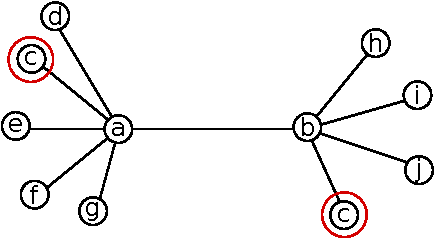
\includegraphics[scale=1]{incidentes}
\caption{Aristas incidentes en $(a,b)$.}
\label{incidencia}
\end{center}
\end{figure}

Si algún $x$ de $(a,x)$ es igual a algún $y$ de $(b,y)$ entonces la arista $(a,b)$ pertenece a un triángulo. En la figura \ref{incidencia} el vértice $c$ es adyacente a $a$ y a $b$, y por lo tanto se forma el triángulo $\{ (a,b), (b,c), (a,c) \}$.

\begin{figure}[htbp]
\begin{center}
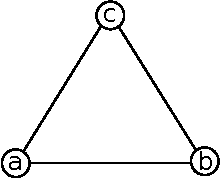
\includegraphics[scale=1]{triangulo}
\caption{Triángulo formado por $a$, $b$ y $c$.}
\label{triangulo}
\end{center}
\end{figure}

Una vez que se encontraron los posibles triángulos para $(a,b)$ hay que aplicar la misma estrategia para el resto de aristas, pero eliminando $(a,b)$ del espacio de búsqueda para evitar triángulos repetidos.

\subsection*{Generando fórmulas}

El programa que traduce una gráfica a una fórmula es \textit{mono\_triangle.hs} y está hecho en Haskell. En mi implementación, una cláusula se representa como una lista de literales, y una forma clausular se representa como una lista de cláusulas. En el archivo \textit{LogicaProp.hs} se encuentra una función que transforma cualquier fórmula a su forma clausular, pero como este problema ya se traduce a 3-FNC no es necesario transformarlo.

Antes de transformar el problema de la gráfica al problema 3-SAT se deben conocer los triángulos de la gráfica. En el módulo \textit{Graph.hs} hay una función (\textit{formaTriangulos3}) que encuentra los triángulos de una gráfica dado su conjunto de aristas. El resultado es una lista de triángulos, y un triángulo está representado con una lista de tres aristas.

Aquí se muestran los pasos para transformar el ejemplar de la gráfica a un ejemplar de 3-SAT:

\begin{itemize}
\item[1.] \textbf{Conjunto de variables.} Primero se transforma el conjunto de aristas a un conjunto de pares de variables proposicionales: para cada arista $(u,v)$ se obtiene el par $(uv1,uv2)$.
\item[2.] \textbf{Mínimo uno.} Para cada par de variables $(uv1, uv2)$ se crea la cláusula $[uv1, uv2]$ que significa $uv_1 \vee uv_2$. Al final se obtiene una lista de cláusulas.
\item[3.] \textbf{Máximo uno.} Para cada par de variables $(uv1, uv2)$ se crea la cláusula $[\neg uv1, \neg uv2]$ que significa $\neg uv_1 \vee \neg uv_2$.
\item[4.] \textbf{Sin triángulos monocromáticos.} Para cada triángulo $[(a,b), (b,c), (c,a)]$ se crean las cláusulas $[\neg ab1, \neg bc1, \neg ca1]$ y $[\neg ab2, \neg bc2, \neg ca2]$.
\item[5.] \textbf{Forma clausular.} Cuando ya se obtuvieron todas las listas de cláusulas se concatenan para crear la forma clausular completa: $minUno ++ maxUno ++ tri$.
\end{itemize}

Ya se tiene la fórmula en forma clausular reconocida por Haskell, ahora hay que traducirla a un formato reconocible por Lisp y guardarlo en un archivo que pueda leer \textbf{z3}.

\begin{itemize}
\item[1.] Para cada variable $x$ se crea la cadena ``\texttt{(declare-const x Bool)}''. Por ejemplo, para la variable $ab1$ se crea ``\texttt{(declare-const ab1 Bool)}''.
\item[2.] Una cláusula es una lista de literales: $[lit_1, lit_2, ..., lit_n]$ y representa una disyunción de literales, así que se crea la cadena ``\texttt{(or lit1 lit2 ... litn)}''. Por ejemplo, para la cláusula $[ab1, ab2]$ se crea ``\texttt{(or ab1 ab2)}''.
\item[3.] Una FNC es una conjunción de cláusulas y se representa con una lista: $[clau_1, clau_2, ... ,clau_n]$. Cada cláusula $clau_i$ se transforma como en 2. y la fórmula total se transforma a la cadena:\\
\texttt{(and\\  (or ...)\\ (or ...)\\ \vdots \\  (or ...))}
\end{itemize}

\section*{Compilación y ejecución}

El código fuente se encuentra en la carpeta \textit{src}. Para compilar se ejecuta el comando \texttt{make}, lo cual genera un ejecutable de \textit{mono\_triangle.hs} y \textit{Visualiza.java}.

Antes de ejecutar, debe haber al menos un archivo de entrada de datos en la carpeta \textit{input}. Una gráfica se codifica de la siguiente forma: en la primera línea hay una cadena de caracteres, y cada caracter será un vértice de la gráfica. De la segunda línea en adelante se tienen pares de caracteres (o sea, cadenas de tamaño dos) que representan las aristas de la gráfica.

Se tomará el archivo \textit{panal} como ejemplo.

Se ejecuta el programa \textit{run.py} con: \texttt{python3 run.py}, lo cual preguntará por el nombre de un archivo, que en este caso es \textit{panal}. Cuando se ejecuta el programa se muestra la lista de cláusulas y luego una gráfica mostrando la partición con azul y rojo. Si la gráfica no tiene una partición, mostrará las aristas de color negro.

\begin{figure}[htbp]
\begin{center}
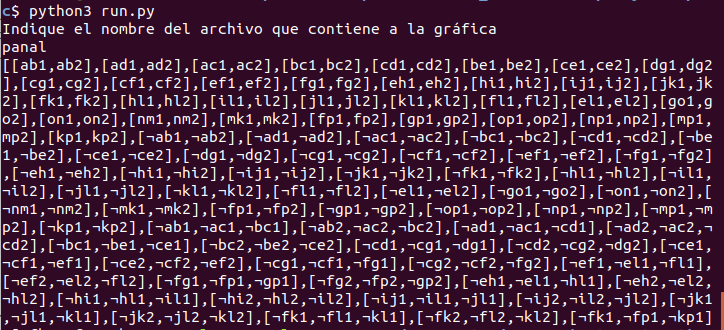
\includegraphics[scale=0.4]{clausulas}
\caption{Forma clausular generada por Haskell.}
\label{fnc}
\end{center}
\end{figure}

\begin{figure}[htbp]
\begin{center}
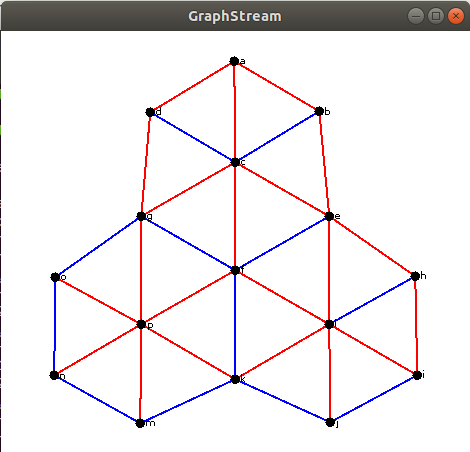
\includegraphics[scale=0.4]{GraphStream}
\caption{Partición de aristas.}
\label{particion}
\end{center}
\end{figure}

La ejecución consta de tres partes:

\begin{itemize}
\item \textbf{Fórmula.} El programa \textit{mono\_triangle} genera una fórmula en un archivo reconocible por z3. El archivo se encuentra en la carpeta \textit{output} y se llama \textit{formula\_panal.smt2}.
\item \textbf{Modelo.} Z3 comprueba si la fórmula generada es satisfacible. Si es satisfacible genera un modelo y guarda el resultado en un archivo en la carpeta \textit{modelos}. El archivo se llama \textit{modelo\_panal}.
\item \textbf{Gráfica.} El programa \textit{Visualiza.java} muestra la gráfica representada por \textit{panal} y colorea las aristas siempre que exista un modelo.
\end{itemize}

\section*{Sobre los ejemplares}

\begin{itemize}
\item[Panal.] El ejemplar \textit{panal} es una gráfica donde se muestran varios triángulos equiláteros acomodados en un plano. Este caso es satisfacible y probablemente cualquier gráfica plana también lo sea.
\item[K5.] El ejemplar \textit{k5} muestra la gráfica completa de orden 5. Este caso también es satisfacible aunque la gráfica no es plana.
\item[K6.] La gráfica completa de orden 6 es insatisfacible, y por lo tanto cualquier gráfica que contenga a $k_6$ como subgráfica también es insatisfacible. Esto nos dice que $k_5$ es la máxima gráfica completa que tiene la partición especificada por el problema.
\end{itemize}


\end{document}


